\documentclass[1p]{elsarticle_modified}
%\bibliographystyle{elsarticle-num}

%\usepackage[colorlinks]{hyperref}
%\usepackage{abbrmath_seonhwa} %\Abb, \Ascr, \Acal ,\Abf, \Afrak
\usepackage{amsfonts}
\usepackage{amssymb}
\usepackage{amsmath}
\usepackage{amsthm}
\usepackage{scalefnt}
\usepackage{amsbsy}
\usepackage{kotex}
\usepackage{caption}
\usepackage{subfig}
\usepackage{color}
\usepackage{graphicx}
\usepackage{xcolor} %% white, black, red, green, blue, cyan, magenta, yellow
\usepackage{float}
\usepackage{setspace}
\usepackage{hyperref}

\usepackage{tikz}
\usetikzlibrary{arrows}

\usepackage{multirow}
\usepackage{array} % fixed length table
\usepackage{hhline}

%%%%%%%%%%%%%%%%%%%%%
\makeatletter
\renewcommand*\env@matrix[1][\arraystretch]{%
	\edef\arraystretch{#1}%
	\hskip -\arraycolsep
	\let\@ifnextchar\new@ifnextchar
	\array{*\c@MaxMatrixCols c}}
\makeatother %https://tex.stackexchange.com/questions/14071/how-can-i-increase-the-line-spacing-in-a-matrix
%%%%%%%%%%%%%%%

\usepackage[normalem]{ulem}

\newcommand{\msout}[1]{\ifmmode\text{\sout{\ensuremath{#1}}}\else\sout{#1}\fi}
%SOURCE: \msout is \stkout macro in https://tex.stackexchange.com/questions/20609/strikeout-in-math-mode

\newcommand{\cancel}[1]{
	\ifmmode
	{\color{red}\msout{#1}}
	\else
	{\color{red}\sout{#1}}
	\fi
}

\newcommand{\add}[1]{
	{\color{blue}\uwave{#1}}
}

\newcommand{\replace}[2]{
	\ifmmode
	{\color{red}\msout{#1}}{\color{blue}\uwave{#2}}
	\else
	{\color{red}\sout{#1}}{\color{blue}\uwave{#2}}
	\fi
}

\newcommand{\Sol}{\mathcal{S}} %segment
\newcommand{\D}{D} %diagram
\newcommand{\A}{\mathcal{A}} %arc


%%%%%%%%%%%%%%%%%%%%%%%%%%%%%5 test

\def\sl{\operatorname{\textup{SL}}(2,\Cbb)}
\def\psl{\operatorname{\textup{PSL}}(2,\Cbb)}
\def\quan{\mkern 1mu \triangleright \mkern 1mu}

\theoremstyle{definition}
\newtheorem{thm}{Theorem}[section]
\newtheorem{prop}[thm]{Proposition}
\newtheorem{lem}[thm]{Lemma}
\newtheorem{ques}[thm]{Question}
\newtheorem{cor}[thm]{Corollary}
\newtheorem{defn}[thm]{Definition}
\newtheorem{exam}[thm]{Example}
\newtheorem{rmk}[thm]{Remark}
\newtheorem{alg}[thm]{Algorithm}

\newcommand{\I}{\sqrt{-1}}
\begin{document}

%\begin{frontmatter}
%
%\title{Boundary parabolic representations of knots up to 8 crossings}
%
%%% Group authors per affiliation:
%\author{Yunhi Cho} 
%\address{Department of Mathematics, University of Seoul, Seoul, Korea}
%\ead{yhcho@uos.ac.kr}
%
%
%\author{Seonhwa Kim} %\fnref{s_kim}}
%\address{Center for Geometry and Physics, Institute for Basic Science, Pohang, 37673, Korea}
%\ead{ryeona17@ibs.re.kr}
%
%\author{Hyuk Kim}
%\address{Department of Mathematical Sciences, Seoul National University, Seoul 08826, Korea}
%\ead{hyukkim@snu.ac.kr}
%
%\author{Seokbeom Yoon}
%\address{Department of Mathematical Sciences, Seoul National University, Seoul, 08826,  Korea}
%\ead{sbyoon15@snu.ac.kr}
%
%\begin{abstract}
%We find all boundary parabolic representation of knots up to 8 crossings.
%
%\end{abstract}
%\begin{keyword}
%    \MSC[2010] 57M25 
%\end{keyword}
%
%\end{frontmatter}

%\linenumbers
%\tableofcontents
%
\newcommand\colored[1]{\textcolor{white}{\rule[-0.35ex]{0.8em}{1.4ex}}\kern-0.8em\color{red} #1}%
%\newcommand\colored[1]{\textcolor{white}{ #1}\kern-2.17ex	\textcolor{white}{ #1}\kern-1.81ex	\textcolor{white}{ #1}\kern-2.15ex\color{red}#1	}

{\Large $\underline{12n_{0785}~(K12n_{0785})}$}

\setlength{\tabcolsep}{10pt}
\renewcommand{\arraystretch}{1.6}
\vspace{1cm}\begin{tabular}{m{100pt}>{\centering\arraybackslash}m{274pt}}
\multirow{5}{120pt}{
	\centering
	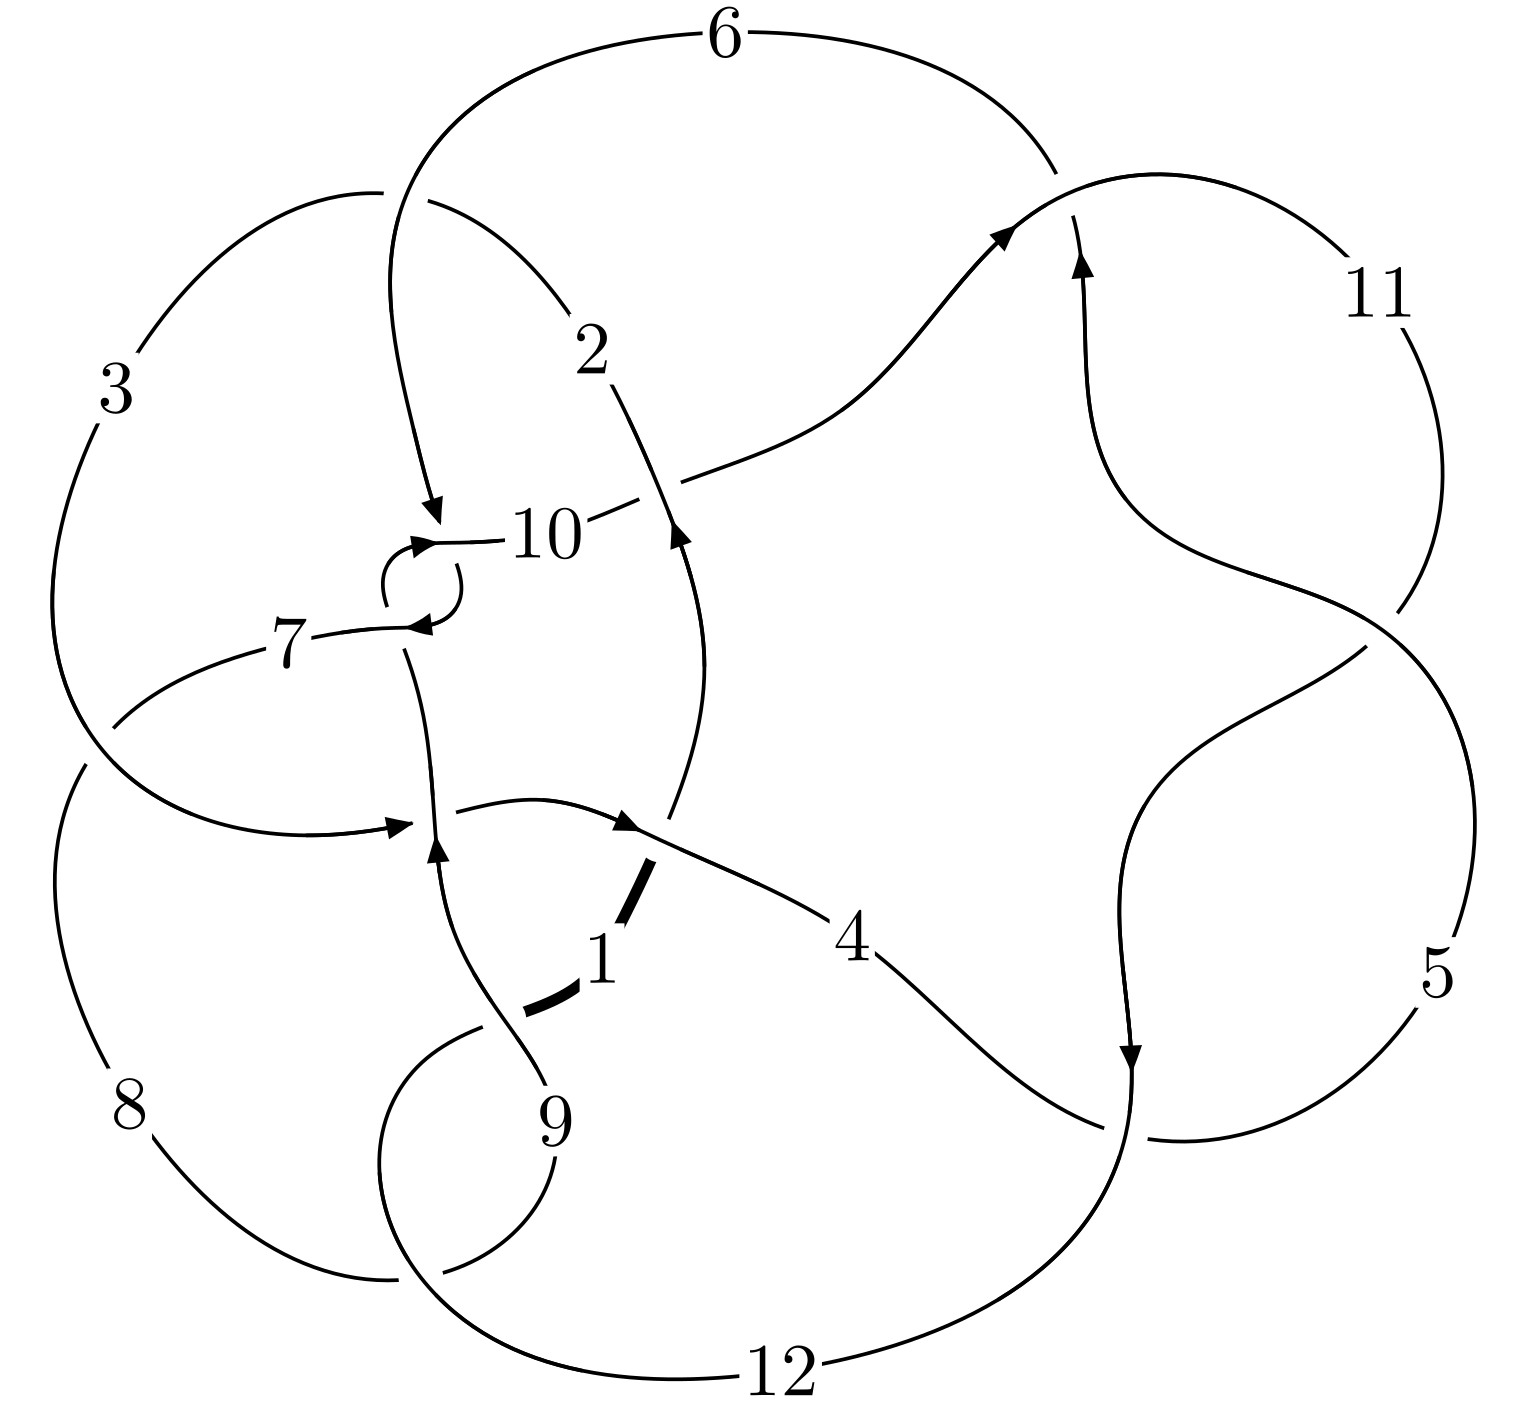
\includegraphics[width=112pt]{../../../GIT/diagram.site/Diagrams/png/2874_12n_0785.png}\\
\ \ \ A knot diagram\footnotemark}&
\allowdisplaybreaks
\textbf{Linearized knot diagam} \\
\cline{2-2}
 &
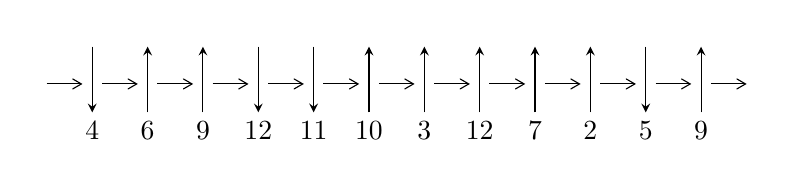
\begin{tikzpicture}[x=20pt, y=17pt]
	% nodes
	\node (C0) at (0, 0) {};
	\node (C1) at (1, 0) {};
	\node (C1U) at (1, +1) {};
	\node (C1D) at (1, -1) {4};

	\node (C2) at (2, 0) {};
	\node (C2U) at (2, +1) {};
	\node (C2D) at (2, -1) {6};

	\node (C3) at (3, 0) {};
	\node (C3U) at (3, +1) {};
	\node (C3D) at (3, -1) {9};

	\node (C4) at (4, 0) {};
	\node (C4U) at (4, +1) {};
	\node (C4D) at (4, -1) {12};

	\node (C5) at (5, 0) {};
	\node (C5U) at (5, +1) {};
	\node (C5D) at (5, -1) {11};

	\node (C6) at (6, 0) {};
	\node (C6U) at (6, +1) {};
	\node (C6D) at (6, -1) {10};

	\node (C7) at (7, 0) {};
	\node (C7U) at (7, +1) {};
	\node (C7D) at (7, -1) {3};

	\node (C8) at (8, 0) {};
	\node (C8U) at (8, +1) {};
	\node (C8D) at (8, -1) {12};

	\node (C9) at (9, 0) {};
	\node (C9U) at (9, +1) {};
	\node (C9D) at (9, -1) {7};

	\node (C10) at (10, 0) {};
	\node (C10U) at (10, +1) {};
	\node (C10D) at (10, -1) {2};

	\node (C11) at (11, 0) {};
	\node (C11U) at (11, +1) {};
	\node (C11D) at (11, -1) {5};

	\node (C12) at (12, 0) {};
	\node (C12U) at (12, +1) {};
	\node (C12D) at (12, -1) {9};
	\node (C13) at (13, 0) {};

	% arrows
	\draw[->,>={angle 60}]
	(C0) edge (C1) (C1) edge (C2) (C2) edge (C3) (C3) edge (C4) (C4) edge (C5) (C5) edge (C6) (C6) edge (C7) (C7) edge (C8) (C8) edge (C9) (C9) edge (C10) (C10) edge (C11) (C11) edge (C12) (C12) edge (C13) ;	\draw[->,>=stealth]
	(C1U) edge (C1D) (C2D) edge (C2U) (C3D) edge (C3U) (C4U) edge (C4D) (C5U) edge (C5D) (C6D) edge (C6U) (C7D) edge (C7U) (C8D) edge (C8U) (C9D) edge (C9U) (C10D) edge (C10U) (C11U) edge (C11D) (C12D) edge (C12U) ;
	\end{tikzpicture} \\
\hhline{~~} \\& 
\textbf{Solving Sequence} \\ \cline{2-2} 
 &
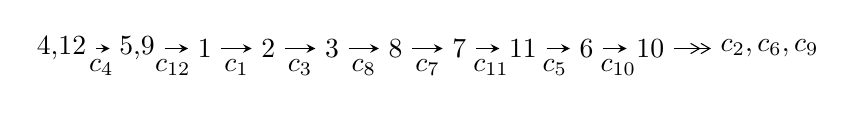
\begin{tikzpicture}[x=23pt, y=7pt]
	% node
	\node (A0) at (-1/8, 0) {4,12};
	\node (A1) at (17/16, 0) {5,9};
	\node (A2) at (17/8, 0) {1};
	\node (A3) at (25/8, 0) {2};
	\node (A4) at (33/8, 0) {3};
	\node (A5) at (41/8, 0) {8};
	\node (A6) at (49/8, 0) {7};
	\node (A7) at (57/8, 0) {11};
	\node (A8) at (65/8, 0) {6};
	\node (A9) at (73/8, 0) {10};
	\node (C1) at (1/2, -1) {$c_{4}$};
	\node (C2) at (13/8, -1) {$c_{12}$};
	\node (C3) at (21/8, -1) {$c_{1}$};
	\node (C4) at (29/8, -1) {$c_{3}$};
	\node (C5) at (37/8, -1) {$c_{8}$};
	\node (C6) at (45/8, -1) {$c_{7}$};
	\node (C7) at (53/8, -1) {$c_{11}$};
	\node (C8) at (61/8, -1) {$c_{5}$};
	\node (C9) at (69/8, -1) {$c_{10}$};
	\node (A10) at (11, 0) {$c_{2},c_{6},c_{9}$};

	% edge
	\draw[->,>=stealth]	
	(A0) edge (A1) (A1) edge (A2) (A2) edge (A3) (A3) edge (A4) (A4) edge (A5) (A5) edge (A6) (A6) edge (A7) (A7) edge (A8) (A8) edge (A9) ;
	\draw[->>,>={angle 60}]	
	(A9) edge (A10);
\end{tikzpicture} \\ 

\end{tabular} \\

\footnotetext{
The image of knot diagram is generated by the software ``\textbf{Draw programme}" developed by Andrew Bartholomew(\url{http://www.layer8.co.uk/maths/draw/index.htm\#Running-draw}), where we modified some parts for our purpose(\url{https://github.com/CATsTAILs/LinksPainter}).
}\phantom \\ \newline 
\centering \textbf{Ideals for irreducible components\footnotemark of $X_{\text{par}}$} 
 
\begin{align*}
I^u_{1}&=\langle 
-27 u^{23}-304 u^{22}+\cdots+32 b-800,\;-25 u^{23}-246 u^{22}+\cdots+64 a+5312,\\
\phantom{I^u_{1}}&\phantom{= \langle  }u^{24}+12 u^{23}+\cdots+736 u+64\rangle \\
I^u_{2}&=\langle 
1.86388\times10^{20} a^{11} u^{2}-7.50093\times10^{19} a^{10} u^{2}+\cdots+1.24248\times10^{20} a+1.90879\times10^{20},\\
\phantom{I^u_{2}}&\phantom{= \langle  }- a^{11} u^2+13 a^{10} u^2+\cdots+2212 a+924,\;u^3- u^2+2 u-1\rangle \\
I^u_{3}&=\langle 
u^{13}+u^{12}+8 u^{11}+6 u^{10}+24 u^9+14 u^8+32 u^7+17 u^6+15 u^5+12 u^4- u^3+4 u^2+b+2 u,\\
\phantom{I^u_{3}}&\phantom{= \langle  }u^{12}+u^{11}+8 u^{10}+6 u^9+24 u^8+14 u^7+32 u^6+17 u^5+15 u^4+12 u^3- u^2+a+4 u+2,\\
\phantom{I^u_{3}}&\phantom{= \langle  }u^{15}+u^{14}+10 u^{13}+8 u^{12}+40 u^{11}+26 u^{10}+80 u^9+44 u^8+78 u^7+40 u^6+25 u^5+16 u^4-5 u^3+2 u+1\rangle \\
\\
\end{align*}
\raggedright * 3 irreducible components of $\dim_{\mathbb{C}}=0$, with total 75 representations.\\
\footnotetext{All coefficients of polynomials are rational numbers. But the coefficients are sometimes approximated in decimal forms when there is not enough margin.}
\newpage
\renewcommand{\arraystretch}{1}
\centering \section*{I. $I^u_{1}= \langle -27 u^{23}-304 u^{22}+\cdots+32 b-800,\;-25 u^{23}-246 u^{22}+\cdots+64 a+5312,\;u^{24}+12 u^{23}+\cdots+736 u+64 \rangle$}
\flushleft \textbf{(i) Arc colorings}\\
\begin{tabular}{m{7pt} m{180pt} m{7pt} m{180pt} }
\flushright $a_{4}=$&$\begin{pmatrix}1\\0\end{pmatrix}$ \\
\flushright $a_{12}=$&$\begin{pmatrix}0\\u\end{pmatrix}$ \\
\flushright $a_{5}=$&$\begin{pmatrix}1\\u^2\end{pmatrix}$ \\
\flushright $a_{9}=$&$\begin{pmatrix}\frac{25}{64} u^{23}+\frac{123}{32} u^{22}+\cdots-\frac{2843}{4} u-83\\\frac{27}{32} u^{23}+\frac{19}{2} u^{22}+\cdots+\frac{741}{2} u+25\end{pmatrix}$ \\
\flushright $a_{1}=$&$\begin{pmatrix}- u^{23}-\frac{47}{4} u^{22}+\cdots-1008 u-\frac{191}{2}\\-\frac{1}{4} u^{23}-\frac{7}{2} u^{22}+\cdots-\frac{1279}{2} u-64\end{pmatrix}$ \\
\flushright $a_{2}=$&$\begin{pmatrix}-0.750000 u^{23}-8.25000 u^{22}+\cdots-368.500 u-31.5000\\-\frac{1}{4} u^{23}-\frac{7}{2} u^{22}+\cdots-\frac{1279}{2} u-64\end{pmatrix}$ \\
\flushright $a_{3}=$&$\begin{pmatrix}u^{23}+\frac{47}{4} u^{22}+\cdots+1008 u+\frac{193}{2}\\\frac{1}{4} u^{23}+\frac{7}{2} u^{22}+\cdots+\frac{1281}{2} u+64\end{pmatrix}$ \\
\flushright $a_{8}=$&$\begin{pmatrix}\frac{25}{64} u^{23}+\frac{123}{32} u^{22}+\cdots-\frac{2843}{4} u-83\\\frac{47}{32} u^{23}+\frac{133}{8} u^{22}+\cdots+\frac{1933}{2} u+79\end{pmatrix}$ \\
\flushright $a_{7}=$&$\begin{pmatrix}-\frac{1}{2} u^{23}-\frac{111}{16} u^{22}+\cdots-1654 u-165\\\frac{15}{8} u^{23}+\frac{337}{16} u^{22}+\cdots+868 u+64\end{pmatrix}$ \\
\flushright $a_{11}=$&$\begin{pmatrix}u\\u^3+u\end{pmatrix}$ \\
\flushright $a_{6}=$&$\begin{pmatrix}u^2+1\\u^4+2 u^2\end{pmatrix}$ \\
\flushright $a_{10}=$&$\begin{pmatrix}-\frac{7}{4} u^{23}-\frac{81}{4} u^{22}+\cdots-\frac{6717}{4} u-160\\\frac{5}{4} u^{23}+14 u^{22}+\cdots+601 u+48\end{pmatrix}$\\&\end{tabular}
\flushleft \textbf{(ii) Obstruction class $= -1$}\\~\\
\flushleft \textbf{(iii) Cusp Shapes $= -\frac{1}{2} u^{23}-\frac{23}{4} u^{22}+\cdots-300 u-34$}\\~\\
\newpage\renewcommand{\arraystretch}{1}
\flushleft \textbf{(iv) u-Polynomials at the component}\newline \\
\begin{tabular}{m{50pt}|m{274pt}}
Crossings & \hspace{64pt}u-Polynomials at each crossing \\
\hline $$\begin{aligned}c_{1}\end{aligned}$$&$\begin{aligned}
&u^{24}-19 u^{23}+\cdots-1308 u+680
\end{aligned}$\\
\hline $$\begin{aligned}c_{2},c_{10}\end{aligned}$$&$\begin{aligned}
&u^{24}- u^{23}+\cdots-2 u+1
\end{aligned}$\\
\hline $$\begin{aligned}c_{3},c_{8},c_{12}\end{aligned}$$&$\begin{aligned}
&u^{24}- u^{23}+\cdots- u+1
\end{aligned}$\\
\hline $$\begin{aligned}c_{4},c_{5},c_{11}\end{aligned}$$&$\begin{aligned}
&u^{24}+12 u^{23}+\cdots+736 u+64
\end{aligned}$\\
\hline $$\begin{aligned}c_{6},c_{9}\end{aligned}$$&$\begin{aligned}
&u^{24}+11 u^{23}+\cdots+116 u+8
\end{aligned}$\\
\hline $$\begin{aligned}c_{7}\end{aligned}$$&$\begin{aligned}
&u^{24}+u^{23}+\cdots-38 u+21
\end{aligned}$\\
\hline
\end{tabular}\\~\\
\newpage\renewcommand{\arraystretch}{1}
\flushleft \textbf{(v) Riley Polynomials at the component}\newline \\
\begin{tabular}{m{50pt}|m{274pt}}
Crossings & \hspace{64pt}Riley Polynomials at each crossing \\
\hline $$\begin{aligned}c_{1}\end{aligned}$$&$\begin{aligned}
&y^{24}-23 y^{23}+\cdots-29904 y+462400
\end{aligned}$\\
\hline $$\begin{aligned}c_{2},c_{10}\end{aligned}$$&$\begin{aligned}
&y^{24}+y^{23}+\cdots+16 y+1
\end{aligned}$\\
\hline $$\begin{aligned}c_{3},c_{8},c_{12}\end{aligned}$$&$\begin{aligned}
&y^{24}+31 y^{23}+\cdots+23 y+1
\end{aligned}$\\
\hline $$\begin{aligned}c_{4},c_{5},c_{11}\end{aligned}$$&$\begin{aligned}
&y^{24}+22 y^{23}+\cdots+11264 y+4096
\end{aligned}$\\
\hline $$\begin{aligned}c_{6},c_{9}\end{aligned}$$&$\begin{aligned}
&y^{24}+19 y^{23}+\cdots-464 y+64
\end{aligned}$\\
\hline $$\begin{aligned}c_{7}\end{aligned}$$&$\begin{aligned}
&y^{24}+15 y^{23}+\cdots+3344 y+441
\end{aligned}$\\
\hline
\end{tabular}\\~\\
\newpage\flushleft \textbf{(vi) Complex Volumes and Cusp Shapes}
$$\begin{array}{c|c|c}  
\text{Solutions to }I^u_{1}& \I (\text{vol} + \sqrt{-1}CS) & \text{Cusp shape}\\
 \hline 
\begin{aligned}
u &= -1.010640 + 0.471333 I \\
a &= \phantom{-}0.44326 - 1.53014 I \\
b &= -0.27323 - 1.75534 I\end{aligned}
 & -10.7115 + 10.0939 I & -0.04933 - 6.43639 I \\ \hline\begin{aligned}
u &= -1.010640 - 0.471333 I \\
a &= \phantom{-}0.44326 + 1.53014 I \\
b &= -0.27323 + 1.75534 I\end{aligned}
 & -10.7115 - 10.0939 I & -0.04933 + 6.43639 I \\ \hline\begin{aligned}
u &= -0.503255 + 0.574177 I \\
a &= \phantom{-}0.835381 + 0.150338 I \\
b &= \phantom{-}0.506730 - 0.403999 I\end{aligned}
 & -2.49625 + 3.04099 I & \phantom{-}1.32899 - 3.32840 I \\ \hline\begin{aligned}
u &= -0.503255 - 0.574177 I \\
a &= \phantom{-}0.835381 - 0.150338 I \\
b &= \phantom{-}0.506730 + 0.403999 I\end{aligned}
 & -2.49625 - 3.04099 I & \phantom{-}1.32899 + 3.32840 I \\ \hline\begin{aligned}
u &= -1.180380 + 0.399451 I \\
a &= -0.295273 + 1.321890 I \\
b &= \phantom{-}0.17950 + 1.67829 I\end{aligned}
 & -5.17987 + 4.24750 I & \phantom{-}3.02010 - 8.12803 I \\ \hline\begin{aligned}
u &= -1.180380 - 0.399451 I \\
a &= -0.295273 - 1.321890 I \\
b &= \phantom{-}0.17950 - 1.67829 I\end{aligned}
 & -5.17987 - 4.24750 I & \phantom{-}3.02010 + 8.12803 I \\ \hline\begin{aligned}
u &= -1.004630 + 0.835014 I \\
a &= \phantom{-}0.759653 - 1.021870 I \\
b &= -0.09010 - 1.66092 I\end{aligned}
 & -9.75365 - 3.54379 I & -0.99118 + 4.27014 I \\ \hline\begin{aligned}
u &= -1.004630 - 0.835014 I \\
a &= \phantom{-}0.759653 + 1.021870 I \\
b &= -0.09010 + 1.66092 I\end{aligned}
 & -9.75365 + 3.54379 I & -0.99118 - 4.27014 I \\ \hline\begin{aligned}
u &= -0.308009 + 0.555063 I \\
a &= -0.449528 + 0.382050 I \\
b &= \phantom{-}0.073603 + 0.367191 I\end{aligned}
 & \phantom{-}0.196861 + 1.129420 I & \phantom{-}2.90140 - 6.41925 I \\ \hline\begin{aligned}
u &= -0.308009 - 0.555063 I \\
a &= -0.449528 - 0.382050 I \\
b &= \phantom{-}0.073603 - 0.367191 I\end{aligned}
 & \phantom{-}0.196861 - 1.129420 I & \phantom{-}2.90140 + 6.41925 I\\
 \hline 
 \end{array}$$\newpage$$\begin{array}{c|c|c}  
\text{Solutions to }I^u_{1}& \I (\text{vol} + \sqrt{-1}CS) & \text{Cusp shape}\\
 \hline 
\begin{aligned}
u &= -0.516904 + 0.317864 I \\
a &= -0.256314 - 1.078460 I \\
b &= -0.475294 - 0.475988 I\end{aligned}
 & -3.21746 + 0.49631 I & \phantom{-}0.08904 - 3.40641 I \\ \hline\begin{aligned}
u &= -0.516904 - 0.317864 I \\
a &= -0.256314 + 1.078460 I \\
b &= -0.475294 + 0.475988 I\end{aligned}
 & -3.21746 - 0.49631 I & \phantom{-}0.08904 + 3.40641 I \\ \hline\begin{aligned}
u &= \phantom{-}0.21488 + 1.45533 I \\
a &= -0.517010 + 0.329331 I \\
b &= \phantom{-}0.590380 + 0.681655 I\end{aligned}
 & \phantom{-}1.83425 + 1.78702 I & \phantom{-}1.23481 - 2.86773 I \\ \hline\begin{aligned}
u &= \phantom{-}0.21488 - 1.45533 I \\
a &= -0.517010 - 0.329331 I \\
b &= \phantom{-}0.590380 - 0.681655 I\end{aligned}
 & \phantom{-}1.83425 - 1.78702 I & \phantom{-}1.23481 + 2.86773 I \\ \hline\begin{aligned}
u &= -0.13976 + 1.54947 I \\
a &= -0.236789 - 0.330108 I \\
b &= -0.544586 + 0.320761 I\end{aligned}
 & \phantom{-}4.59873 + 5.35349 I & \phantom{-}4.00000 + 0. I\phantom{ +0.000000I} \\ \hline\begin{aligned}
u &= -0.13976 - 1.54947 I \\
a &= -0.236789 + 0.330108 I \\
b &= -0.544586 - 0.320761 I\end{aligned}
 & \phantom{-}4.59873 - 5.35349 I & \phantom{-}4.00000 + 0. I\phantom{ +0.000000I} \\ \hline\begin{aligned}
u &= -0.10640 + 1.57603 I \\
a &= \phantom{-}0.285679 + 0.026175 I \\
b &= \phantom{-}0.071649 - 0.447453 I\end{aligned}
 & \phantom{-}7.58277 + 2.71010 I & \phantom{-}1.02540 - 3.86743 I \\ \hline\begin{aligned}
u &= -0.10640 - 1.57603 I \\
a &= \phantom{-}0.285679 - 0.026175 I \\
b &= \phantom{-}0.071649 + 0.447453 I\end{aligned}
 & \phantom{-}7.58277 - 2.71010 I & \phantom{-}1.02540 + 3.86743 I \\ \hline\begin{aligned}
u &= -0.43383 + 1.51943 I \\
a &= \phantom{-}0.868418 - 0.623221 I \\
b &= -0.57020 - 1.58987 I\end{aligned}
 & \phantom{-}0.89209 + 9.87509 I & \phantom{-}6.51442 - 6.39656 I \\ \hline\begin{aligned}
u &= -0.43383 - 1.51943 I \\
a &= \phantom{-}0.868418 + 0.623221 I \\
b &= -0.57020 + 1.58987 I\end{aligned}
 & \phantom{-}0.89209 - 9.87509 I & \phantom{-}6.51442 + 6.39656 I\\
 \hline 
 \end{array}$$\newpage$$\begin{array}{c|c|c}  
\text{Solutions to }I^u_{1}& \I (\text{vol} + \sqrt{-1}CS) & \text{Cusp shape}\\
 \hline 
\begin{aligned}
u &= -0.39076 + 1.53782 I \\
a &= -0.947929 + 0.618450 I \\
b &= \phantom{-}0.58065 + 1.69940 I\end{aligned}
 & -4.2980 + 15.1741 I & \phantom{-}4.00000 - 7.27803 I \\ \hline\begin{aligned}
u &= -0.39076 - 1.53782 I \\
a &= -0.947929 - 0.618450 I \\
b &= \phantom{-}0.58065 - 1.69940 I\end{aligned}
 & -4.2980 - 15.1741 I & \phantom{-}4.00000 + 7.27803 I \\ \hline\begin{aligned}
u &= -0.62030 + 1.53231 I \\
a &= -0.739547 + 0.593643 I \\
b &= \phantom{-}0.45090 + 1.50145 I\end{aligned}
 & -1.65465 + 3.46994 I & \phantom{-}7.08633 - 7.90223 I \\ \hline\begin{aligned}
u &= -0.62030 - 1.53231 I \\
a &= -0.739547 - 0.593643 I \\
b &= \phantom{-}0.45090 - 1.50145 I\end{aligned}
 & -1.65465 - 3.46994 I & \phantom{-}7.08633 + 7.90223 I\\
 \hline 
 \end{array}$$\newpage\newpage\renewcommand{\arraystretch}{1}
\centering \section*{II. $I^u_{2}= \langle 1.86\times10^{20} a^{11} u^{2}-7.50\times10^{19} a^{10} u^{2}+\cdots+1.24\times10^{20} a+1.91\times10^{20},\;- a^{11} u^2+13 a^{10} u^2+\cdots+2212 a+924,\;u^3- u^2+2 u-1 \rangle$}
\flushleft \textbf{(i) Arc colorings}\\
\begin{tabular}{m{7pt} m{180pt} m{7pt} m{180pt} }
\flushright $a_{4}=$&$\begin{pmatrix}1\\0\end{pmatrix}$ \\
\flushright $a_{12}=$&$\begin{pmatrix}0\\u\end{pmatrix}$ \\
\flushright $a_{5}=$&$\begin{pmatrix}1\\u^2\end{pmatrix}$ \\
\flushright $a_{9}=$&$\begin{pmatrix}a\\-3.24277 a^{11} u^{2}+1.30501 a^{10} u^{2}+\cdots-2.16165 a-3.32090\end{pmatrix}$ \\
\flushright $a_{1}=$&$\begin{pmatrix}a^2 u\\-0.581414 a^{11} u^{2}+3.43653 a^{10} u^{2}+\cdots-7.52437 a-2.00296\end{pmatrix}$ \\
\flushright $a_{2}=$&$\begin{pmatrix}0.581414 a^{11} u^{2}-3.43653 a^{10} u^{2}+\cdots+7.52437 a+2.00296\\-0.581414 a^{11} u^{2}+3.43653 a^{10} u^{2}+\cdots-7.52437 a-2.00296\end{pmatrix}$ \\
\flushright $a_{3}=$&$\begin{pmatrix}3.13144 a^{11} u^{2}+0.478770 a^{10} u^{2}+\cdots-1.90212 a+2.66819\\-6.90860 a^{11} u^{2}+7.51166 a^{10} u^{2}+\cdots-16.6685 a-8.90871\end{pmatrix}$ \\
\flushright $a_{8}=$&$\begin{pmatrix}a\\-3.24277 a^{11} u^{2}+1.30501 a^{10} u^{2}+\cdots-2.16165 a-3.32090\end{pmatrix}$ \\
\flushright $a_{7}=$&$\begin{pmatrix}-1.35924 a^{11} u^{2}-0.912568 a^{10} u^{2}+\cdots+2.14523 a-1.30624\\0.862884 a^{11} u^{2}-3.85601 a^{10} u^{2}+\cdots+6.58457 a+2.47234\end{pmatrix}$ \\
\flushright $a_{11}=$&$\begin{pmatrix}u\\u^2- u+1\end{pmatrix}$ \\
\flushright $a_{6}=$&$\begin{pmatrix}u^2+1\\u^2- u+1\end{pmatrix}$ \\
\flushright $a_{10}=$&$\begin{pmatrix}1.44285 a^{11} u^{2}-0.692279 a^{10} u^{2}+\cdots+1.99663 a+1.48796\\2.28994 a^{11} u^{2}+0.187392 a^{10} u^{2}+\cdots-0.897794 a+2.62937\end{pmatrix}$\\&\end{tabular}
\flushleft \textbf{(ii) Obstruction class $= -1$}\\~\\
\flushleft \textbf{(iii) Cusp Shapes $= -\frac{739013742275411059680}{57478066342067795059} a^{11} u^2+\frac{40574843941814876112}{57478066342067795059} a^{10} u^2+\cdots+\frac{328493151198246771284}{57478066342067795059} a-\frac{454117950256466456506}{57478066342067795059}$}\\~\\
\newpage\renewcommand{\arraystretch}{1}
\flushleft \textbf{(iv) u-Polynomials at the component}\newline \\
\begin{tabular}{m{50pt}|m{274pt}}
Crossings & \hspace{64pt}u-Polynomials at each crossing \\
\hline $$\begin{aligned}c_{1}\end{aligned}$$&$\begin{aligned}
&(u^6+5 u^5+7 u^4-2 u^2+3 u-1)^6
\end{aligned}$\\
\hline $$\begin{aligned}c_{2},c_{10}\end{aligned}$$&$\begin{aligned}
&u^{36}-5 u^{35}+\cdots+8 u-1
\end{aligned}$\\
\hline $$\begin{aligned}c_{3},c_{8},c_{12}\end{aligned}$$&$\begin{aligned}
&u^{36}- u^{35}+\cdots-7944 u+1231
\end{aligned}$\\
\hline $$\begin{aligned}c_{4},c_{5},c_{11}\end{aligned}$$&$\begin{aligned}
&(u^3- u^2+2 u-1)^{12}
\end{aligned}$\\
\hline $$\begin{aligned}c_{6},c_{9}\end{aligned}$$&$\begin{aligned}
&(u^6- u^5+3 u^4-2 u^3+2 u^2- u-1)^6
\end{aligned}$\\
\hline $$\begin{aligned}c_{7}\end{aligned}$$&$\begin{aligned}
&u^{36}+u^{35}+\cdots+4818 u-3979
\end{aligned}$\\
\hline
\end{tabular}\\~\\
\newpage\renewcommand{\arraystretch}{1}
\flushleft \textbf{(v) Riley Polynomials at the component}\newline \\
\begin{tabular}{m{50pt}|m{274pt}}
Crossings & \hspace{64pt}Riley Polynomials at each crossing \\
\hline $$\begin{aligned}c_{1}\end{aligned}$$&$\begin{aligned}
&(y^6-11 y^5+45 y^4-60 y^3-10 y^2-5 y+1)^6
\end{aligned}$\\
\hline $$\begin{aligned}c_{2},c_{10}\end{aligned}$$&$\begin{aligned}
&y^{36}-5 y^{35}+\cdots+2420 y^2+1
\end{aligned}$\\
\hline $$\begin{aligned}c_{3},c_{8},c_{12}\end{aligned}$$&$\begin{aligned}
&y^{36}+35 y^{35}+\cdots-8165144 y+1515361
\end{aligned}$\\
\hline $$\begin{aligned}c_{4},c_{5},c_{11}\end{aligned}$$&$\begin{aligned}
&(y^3+3 y^2+2 y-1)^{12}
\end{aligned}$\\
\hline $$\begin{aligned}c_{6},c_{9}\end{aligned}$$&$\begin{aligned}
&(y^6+5 y^5+9 y^4+4 y^3-6 y^2-5 y+1)^6
\end{aligned}$\\
\hline $$\begin{aligned}c_{7}\end{aligned}$$&$\begin{aligned}
&y^{36}+23 y^{35}+\cdots-900566708 y+15832441
\end{aligned}$\\
\hline
\end{tabular}\\~\\
\newpage\flushleft \textbf{(vi) Complex Volumes and Cusp Shapes}
$$\begin{array}{c|c|c}  
\text{Solutions to }I^u_{2}& \I (\text{vol} + \sqrt{-1}CS) & \text{Cusp shape}\\
 \hline 
\begin{aligned}
u &= \phantom{-}0.215080 + 1.307140 I \\
a &= \phantom{-}0.292445 - 0.976914 I \\
b &= -0.010553 - 0.974222 I\end{aligned}
 & \phantom{-}5.74941 - 2.82812 I & \phantom{-}7.77925 + 2.97945 I \\ \hline\begin{aligned}
u &= \phantom{-}0.215080 + 1.307140 I \\
a &= \phantom{-}0.879256 + 0.628433 I \\
b &= -0.20795 + 1.64474 I\end{aligned}
 & -1.17182 - 2.82812 I & \phantom{-}8.92653 + 2.97945 I \\ \hline\begin{aligned}
u &= \phantom{-}0.215080 + 1.307140 I \\
a &= -0.835208 - 0.315914 I \\
b &= \phantom{-}0.22908 - 2.03181 I\end{aligned}
 & -4.87092 - 0.85571 I & \phantom{-}0.085479 - 0.705331 I \\ \hline\begin{aligned}
u &= \phantom{-}0.215080 + 1.307140 I \\
a &= -0.818019 - 0.239393 I \\
b &= \phantom{-}1.59293 - 0.13103 I\end{aligned}
 & \phantom{-}1.78490 - 7.42025 I & \phantom{-}4.09089 + 6.18427 I \\ \hline\begin{aligned}
u &= \phantom{-}0.215080 + 1.307140 I \\
a &= \phantom{-}1.103510 + 0.320281 I \\
b &= -1.04255 + 1.64876 I\end{aligned}
 & -4.87092 - 4.80053 I & \phantom{-}0.08548 + 6.66423 I \\ \hline\begin{aligned}
u &= \phantom{-}0.215080 + 1.307140 I \\
a &= -0.097635 + 1.202570 I \\
b &= -0.136981 + 1.120760 I\end{aligned}
 & \phantom{-}1.78490 - 7.42025 I & \phantom{-}4.09089 + 6.18427 I \\ \hline\begin{aligned}
u &= \phantom{-}0.215080 + 1.307140 I \\
a &= -1.199620 - 0.356474 I \\
b &= \phantom{-}0.63234 - 1.28448 I\end{aligned}
 & -1.17182 - 2.82812 I & \phantom{-}8.92653 + 2.97945 I \\ \hline\begin{aligned}
u &= \phantom{-}0.215080 + 1.307140 I \\
a &= -0.505561 + 0.535105 I \\
b &= \phantom{-}0.404790 + 0.730191 I\end{aligned}
 & \phantom{-}1.78490 + 1.76400 I & \phantom{-}4.09089 - 0.22537 I \\ \hline\begin{aligned}
u &= \phantom{-}0.215080 + 1.307140 I \\
a &= \phantom{-}0.726954 + 0.111541 I \\
b &= -1.339860 - 0.172152 I\end{aligned}
 & \phantom{-}5.74941 - 2.82812 I & \phantom{-}7.77925 + 2.97945 I \\ \hline\begin{aligned}
u &= \phantom{-}0.215080 + 1.307140 I \\
a &= -0.593503 + 0.212019 I \\
b &= \phantom{-}0.808193 + 0.545750 I\end{aligned}
 & \phantom{-}1.78490 + 1.76400 I & \phantom{-}4.09089 - 0.22537 I\\
 \hline 
 \end{array}$$\newpage$$\begin{array}{c|c|c}  
\text{Solutions to }I^u_{2}& \I (\text{vol} + \sqrt{-1}CS) & \text{Cusp shape}\\
 \hline 
\begin{aligned}
u &= \phantom{-}0.215080 + 1.307140 I \\
a &= -1.10032 - 0.97863 I \\
b &= \phantom{-}0.18131 - 1.51133 I\end{aligned}
 & -4.87092 - 4.80053 I & \phantom{-}0.08548 + 6.66423 I \\ \hline\begin{aligned}
u &= \phantom{-}0.215080 + 1.307140 I \\
a &= \phantom{-}1.48534 + 0.41966 I \\
b &= -0.233308 + 1.159680 I\end{aligned}
 & -4.87092 - 0.85571 I & \phantom{-}0.085479 - 0.705331 I \\ \hline\begin{aligned}
u &= \phantom{-}0.215080 - 1.307140 I \\
a &= \phantom{-}0.292445 + 0.976914 I \\
b &= -0.010553 + 0.974222 I\end{aligned}
 & \phantom{-}5.74941 + 2.82812 I & \phantom{-}7.77925 - 2.97945 I \\ \hline\begin{aligned}
u &= \phantom{-}0.215080 - 1.307140 I \\
a &= \phantom{-}0.879256 - 0.628433 I \\
b &= -0.20795 - 1.64474 I\end{aligned}
 & -1.17182 + 2.82812 I & \phantom{-}8.92653 - 2.97945 I \\ \hline\begin{aligned}
u &= \phantom{-}0.215080 - 1.307140 I \\
a &= -0.835208 + 0.315914 I \\
b &= \phantom{-}0.22908 + 2.03181 I\end{aligned}
 & -4.87092 + 0.85571 I & \phantom{-}0.085479 + 0.705331 I \\ \hline\begin{aligned}
u &= \phantom{-}0.215080 - 1.307140 I \\
a &= -0.818019 + 0.239393 I \\
b &= \phantom{-}1.59293 + 0.13103 I\end{aligned}
 & \phantom{-}1.78490 + 7.42025 I & \phantom{-}4.09089 - 6.18427 I \\ \hline\begin{aligned}
u &= \phantom{-}0.215080 - 1.307140 I \\
a &= \phantom{-}1.103510 - 0.320281 I \\
b &= -1.04255 - 1.64876 I\end{aligned}
 & -4.87092 + 4.80053 I & \phantom{-}0.08548 - 6.66423 I \\ \hline\begin{aligned}
u &= \phantom{-}0.215080 - 1.307140 I \\
a &= -0.097635 - 1.202570 I \\
b &= -0.136981 - 1.120760 I\end{aligned}
 & \phantom{-}1.78490 + 7.42025 I & \phantom{-}4.09089 - 6.18427 I \\ \hline\begin{aligned}
u &= \phantom{-}0.215080 - 1.307140 I \\
a &= -1.199620 + 0.356474 I \\
b &= \phantom{-}0.63234 + 1.28448 I\end{aligned}
 & -1.17182 + 2.82812 I & \phantom{-}8.92653 - 2.97945 I \\ \hline\begin{aligned}
u &= \phantom{-}0.215080 - 1.307140 I \\
a &= -0.505561 - 0.535105 I \\
b &= \phantom{-}0.404790 - 0.730191 I\end{aligned}
 & \phantom{-}1.78490 - 1.76400 I & \phantom{-}4.09089 + 0.22537 I\\
 \hline 
 \end{array}$$\newpage$$\begin{array}{c|c|c}  
\text{Solutions to }I^u_{2}& \I (\text{vol} + \sqrt{-1}CS) & \text{Cusp shape}\\
 \hline 
\begin{aligned}
u &= \phantom{-}0.215080 - 1.307140 I \\
a &= \phantom{-}0.726954 - 0.111541 I \\
b &= -1.339860 + 0.172152 I\end{aligned}
 & \phantom{-}5.74941 + 2.82812 I & \phantom{-}7.77925 - 2.97945 I \\ \hline\begin{aligned}
u &= \phantom{-}0.215080 - 1.307140 I \\
a &= -0.593503 - 0.212019 I \\
b &= \phantom{-}0.808193 - 0.545750 I\end{aligned}
 & \phantom{-}1.78490 - 1.76400 I & \phantom{-}4.09089 + 0.22537 I \\ \hline\begin{aligned}
u &= \phantom{-}0.215080 - 1.307140 I \\
a &= -1.10032 + 0.97863 I \\
b &= \phantom{-}0.18131 + 1.51133 I\end{aligned}
 & -4.87092 + 4.80053 I & \phantom{-}0.08548 - 6.66423 I \\ \hline\begin{aligned}
u &= \phantom{-}0.215080 - 1.307140 I \\
a &= \phantom{-}1.48534 - 0.41966 I \\
b &= -0.233308 - 1.159680 I\end{aligned}
 & -4.87092 + 0.85571 I & \phantom{-}0.085479 + 0.705331 I \\ \hline\begin{aligned}
u &= \phantom{-}0.569840\phantom{ +0.000000I} \\
a &= \phantom{-}0.037672 + 0.791957 I \\
b &= -1.126600 + 0.574406 I\end{aligned}
 & -2.35268 - 4.59213 I & -2.43837 + 3.20482 I \\ \hline\begin{aligned}
u &= \phantom{-}0.569840\phantom{ +0.000000I} \\
a &= \phantom{-}0.037672 - 0.791957 I \\
b &= -1.126600 - 0.574406 I\end{aligned}
 & -2.35268 + 4.59213 I & -2.43837 - 3.20482 I \\ \hline\begin{aligned}
u &= \phantom{-}0.569840\phantom{ +0.000000I} \\
a &= -0.371632\phantom{ +0.000000I} \\
b &= \phantom{-}0.950019\phantom{ +0.000000I}\end{aligned}
 & \phantom{-}1.61183\phantom{ +0.000000I} & \phantom{-}1.25000\phantom{ +0.000000I} \\ \hline\begin{aligned}
u &= \phantom{-}0.569840\phantom{ +0.000000I} \\
a &= -1.66717\phantom{ +0.000000I} \\
b &= \phantom{-}0.211771\phantom{ +0.000000I}\end{aligned}
 & \phantom{-}1.61183\phantom{ +0.000000I} & \phantom{-}1.25000\phantom{ +0.000000I} \\ \hline\begin{aligned}
u &= \phantom{-}0.569840\phantom{ +0.000000I} \\
a &= \phantom{-}1.97705 + 1.00801 I \\
b &= -0.021467 + 0.451289 I\end{aligned}
 & -2.35268 + 4.59213 I & -2.43837 - 3.20482 I \\ \hline\begin{aligned}
u &= \phantom{-}0.569840\phantom{ +0.000000I} \\
a &= \phantom{-}1.97705 - 1.00801 I \\
b &= -0.021467 - 0.451289 I\end{aligned}
 & -2.35268 - 4.59213 I & -2.43837 + 3.20482 I\\
 \hline 
 \end{array}$$\newpage$$\begin{array}{c|c|c}  
\text{Solutions to }I^u_{2}& \I (\text{vol} + \sqrt{-1}CS) & \text{Cusp shape}\\
 \hline 
\begin{aligned}
u &= \phantom{-}0.569840\phantom{ +0.000000I} \\
a &= \phantom{-}0.01895 + 2.50724 I \\
b &= \phantom{-}0.38309 + 1.86300 I\end{aligned}
 & -9.00850 + 1.97241 I & -6.44379 - 3.68478 I \\ \hline\begin{aligned}
u &= \phantom{-}0.569840\phantom{ +0.000000I} \\
a &= \phantom{-}0.01895 - 2.50724 I \\
b &= \phantom{-}0.38309 - 1.86300 I\end{aligned}
 & -9.00850 - 1.97241 I & -6.44379 + 3.68478 I \\ \hline\begin{aligned}
u &= \phantom{-}0.569840\phantom{ +0.000000I} \\
a &= \phantom{-}0.32036 + 2.66289 I \\
b &= -0.18256 + 1.51742 I\end{aligned}
 & -5.30941\phantom{ +0.000000I} & \phantom{-}2.39727 + 0. I\phantom{ +0.000000I} \\ \hline\begin{aligned}
u &= \phantom{-}0.569840\phantom{ +0.000000I} \\
a &= \phantom{-}0.32036 - 2.66289 I \\
b &= -0.18256 - 1.51742 I\end{aligned}
 & -5.30941\phantom{ +0.000000I} & \phantom{-}2.39727 + 0. I\phantom{ +0.000000I} \\ \hline\begin{aligned}
u &= \phantom{-}0.569840\phantom{ +0.000000I} \\
a &= -0.67227 + 3.26933 I \\
b &= -0.01080 + 1.42872 I\end{aligned}
 & -9.00850 - 1.97241 I & -6.44379 + 3.68478 I \\ \hline\begin{aligned}
u &= \phantom{-}0.569840\phantom{ +0.000000I} \\
a &= -0.67227 - 3.26933 I \\
b &= -0.01080 - 1.42872 I\end{aligned}
 & -9.00850 + 1.97241 I & -6.44379 - 3.68478 I\\
 \hline 
 \end{array}$$\newpage\newpage\renewcommand{\arraystretch}{1}
\centering \section*{III. $I^u_{3}= \langle u^{13}+u^{12}+\cdots+b+2 u,\;u^{12}+u^{11}+\cdots+a+2,\;u^{15}+u^{14}+\cdots+2 u+1 \rangle$}
\flushleft \textbf{(i) Arc colorings}\\
\begin{tabular}{m{7pt} m{180pt} m{7pt} m{180pt} }
\flushright $a_{4}=$&$\begin{pmatrix}1\\0\end{pmatrix}$ \\
\flushright $a_{12}=$&$\begin{pmatrix}0\\u\end{pmatrix}$ \\
\flushright $a_{5}=$&$\begin{pmatrix}1\\u^2\end{pmatrix}$ \\
\flushright $a_{9}=$&$\begin{pmatrix}- u^{12}- u^{11}+\cdots-4 u-2\\- u^{13}- u^{12}+\cdots-4 u^2-2 u\end{pmatrix}$ \\
\flushright $a_{1}=$&$\begin{pmatrix}u^{13}+u^{12}+\cdots-2 u-1\\u^{14}+u^{13}+\cdots+8 u^3-2 u^2\end{pmatrix}$ \\
\flushright $a_{2}=$&$\begin{pmatrix}- u^{14}-8 u^{12}+\cdots-2 u-1\\u^{14}+u^{13}+\cdots+8 u^3-2 u^2\end{pmatrix}$ \\
\flushright $a_{3}=$&$\begin{pmatrix}u^{13}+u^{12}+\cdots+8 u^2-2 u\\u^{14}+u^{13}+\cdots-2 u^2- u\end{pmatrix}$ \\
\flushright $a_{8}=$&$\begin{pmatrix}- u^{12}- u^{11}+\cdots-4 u-2\\- u^{14}-2 u^{13}+\cdots-6 u^2-2 u\end{pmatrix}$ \\
\flushright $a_{7}=$&$\begin{pmatrix}- u^{14}-10 u^{12}+\cdots+4 u-1\\- u^{10}- u^9-6 u^8-4 u^7-12 u^6-5 u^5-7 u^4- u^3+4 u^2+2 u+1\end{pmatrix}$ \\
\flushright $a_{11}=$&$\begin{pmatrix}u\\u^3+u\end{pmatrix}$ \\
\flushright $a_{6}=$&$\begin{pmatrix}u^2+1\\u^4+2 u^2\end{pmatrix}$ \\
\flushright $a_{10}=$&$\begin{pmatrix}u^{12}+8 u^{10}+26 u^8+u^7+40 u^6+6 u^5+24 u^4+12 u^3- u^2+6 u\\u^{11}+u^{10}+7 u^9+5 u^8+18 u^7+10 u^6+20 u^5+10 u^4+7 u^3+4 u^2\end{pmatrix}$\\&\end{tabular}
\flushleft \textbf{(ii) Obstruction class $= 1$}\\~\\
\flushleft \textbf{(iii) Cusp Shapes $= -2 u^{14}-4 u^{13}-18 u^{12}-27 u^{11}-62 u^{10}-71 u^9-103 u^8-86 u^7-78 u^6-42 u^5-9 u^4-10 u^3+17 u^2-12 u+3$}\\~\\
\newpage\renewcommand{\arraystretch}{1}
\flushleft \textbf{(iv) u-Polynomials at the component}\newline \\
\begin{tabular}{m{50pt}|m{274pt}}
Crossings & \hspace{64pt}u-Polynomials at each crossing \\
\hline $$\begin{aligned}c_{1}\end{aligned}$$&$\begin{aligned}
&u^{15}-12 u^{14}+\cdots+106 u-7
\end{aligned}$\\
\hline $$\begin{aligned}c_{2},c_{10}\end{aligned}$$&$\begin{aligned}
&u^{15}- u^{14}+\cdots-3 u+1
\end{aligned}$\\
\hline $$\begin{aligned}c_{3},c_{8}\end{aligned}$$&$\begin{aligned}
&u^{15}+u^{14}+\cdots-5 u^2+1
\end{aligned}$\\
\hline $$\begin{aligned}c_{4},c_{5}\end{aligned}$$&$\begin{aligned}
&u^{15}+u^{14}+\cdots+2 u+1
\end{aligned}$\\
\hline $$\begin{aligned}c_{6}\end{aligned}$$&$\begin{aligned}
&u^{15}+4 u^{14}+\cdots+16 u+5
\end{aligned}$\\
\hline $$\begin{aligned}c_{7}\end{aligned}$$&$\begin{aligned}
&u^{15}- u^{14}+\cdots+19 u-13
\end{aligned}$\\
\hline $$\begin{aligned}c_{9}\end{aligned}$$&$\begin{aligned}
&u^{15}-4 u^{14}+\cdots+16 u-5
\end{aligned}$\\
\hline $$\begin{aligned}c_{11}\end{aligned}$$&$\begin{aligned}
&u^{15}- u^{14}+\cdots+2 u-1
\end{aligned}$\\
\hline $$\begin{aligned}c_{12}\end{aligned}$$&$\begin{aligned}
&u^{15}- u^{14}+\cdots+5 u^2-1
\end{aligned}$\\
\hline
\end{tabular}\\~\\
\newpage\renewcommand{\arraystretch}{1}
\flushleft \textbf{(v) Riley Polynomials at the component}\newline \\
\begin{tabular}{m{50pt}|m{274pt}}
Crossings & \hspace{64pt}Riley Polynomials at each crossing \\
\hline $$\begin{aligned}c_{1}\end{aligned}$$&$\begin{aligned}
&y^{15}-12 y^{14}+\cdots+5160 y-49
\end{aligned}$\\
\hline $$\begin{aligned}c_{2},c_{10}\end{aligned}$$&$\begin{aligned}
&y^{15}-3 y^{14}+\cdots+13 y-1
\end{aligned}$\\
\hline $$\begin{aligned}c_{3},c_{8},c_{12}\end{aligned}$$&$\begin{aligned}
&y^{15}+11 y^{14}+\cdots+10 y-1
\end{aligned}$\\
\hline $$\begin{aligned}c_{4},c_{5},c_{11}\end{aligned}$$&$\begin{aligned}
&y^{15}+19 y^{14}+\cdots+4 y-1
\end{aligned}$\\
\hline $$\begin{aligned}c_{6},c_{9}\end{aligned}$$&$\begin{aligned}
&y^{15}+14 y^{14}+\cdots-84 y-25
\end{aligned}$\\
\hline $$\begin{aligned}c_{7}\end{aligned}$$&$\begin{aligned}
&y^{15}+11 y^{14}+\cdots+517 y-169
\end{aligned}$\\
\hline
\end{tabular}\\~\\
\newpage\flushleft \textbf{(vi) Complex Volumes and Cusp Shapes}
$$\begin{array}{c|c|c}  
\text{Solutions to }I^u_{3}& \I (\text{vol} + \sqrt{-1}CS) & \text{Cusp shape}\\
 \hline 
\begin{aligned}
u &= \phantom{-}0.323844 + 1.269380 I \\
a &= \phantom{-}1.029620 + 0.553032 I \\
b &= -0.36857 + 1.48607 I\end{aligned}
 & -2.53804 - 2.24615 I & \phantom{-}2.16387 + 0.54553 I \\ \hline\begin{aligned}
u &= \phantom{-}0.323844 - 1.269380 I \\
a &= \phantom{-}1.029620 - 0.553032 I \\
b &= -0.36857 - 1.48607 I\end{aligned}
 & -2.53804 + 2.24615 I & \phantom{-}2.16387 - 0.54553 I \\ \hline\begin{aligned}
u &= \phantom{-}0.144598 + 1.313360 I \\
a &= -1.174410 - 0.519311 I \\
b &= \phantom{-}0.51223 - 1.61751 I\end{aligned}
 & -4.36159 - 3.39759 I & \phantom{-}2.91969 + 0.94976 I \\ \hline\begin{aligned}
u &= \phantom{-}0.144598 - 1.313360 I \\
a &= -1.174410 + 0.519311 I \\
b &= \phantom{-}0.51223 + 1.61751 I\end{aligned}
 & -4.36159 + 3.39759 I & \phantom{-}2.91969 - 0.94976 I \\ \hline\begin{aligned}
u &= -0.648777\phantom{ +0.000000I} \\
a &= \phantom{-}1.14669\phantom{ +0.000000I} \\
b &= -0.743944\phantom{ +0.000000I}\end{aligned}
 & \phantom{-}2.16310\phantom{ +0.000000I} & \phantom{-}19.7840\phantom{ +0.000000I} \\ \hline\begin{aligned}
u &= -0.09083 + 1.51451 I \\
a &= -0.115298 + 0.423871 I \\
b &= -0.631485 - 0.213121 I\end{aligned}
 & \phantom{-}4.83768 + 6.28589 I & \phantom{-}6.55684 - 7.16786 I \\ \hline\begin{aligned}
u &= -0.09083 - 1.51451 I \\
a &= -0.115298 - 0.423871 I \\
b &= -0.631485 + 0.213121 I\end{aligned}
 & \phantom{-}4.83768 - 6.28589 I & \phantom{-}6.55684 + 7.16786 I \\ \hline\begin{aligned}
u &= \phantom{-}0.403094 + 0.263692 I \\
a &= -1.89519 - 2.58749 I \\
b &= -0.08164 - 1.54275 I\end{aligned}
 & -8.01131 + 1.56669 I & \phantom{-}2.47871 - 0.14188 I \\ \hline\begin{aligned}
u &= \phantom{-}0.403094 - 0.263692 I \\
a &= -1.89519 + 2.58749 I \\
b &= -0.08164 + 1.54275 I\end{aligned}
 & -8.01131 - 1.56669 I & \phantom{-}2.47871 + 0.14188 I \\ \hline\begin{aligned}
u &= -0.13670 + 1.53364 I \\
a &= -0.169899 - 0.313484 I \\
b &= \phantom{-}0.503998 - 0.217711 I\end{aligned}
 & \phantom{-}8.19478 + 2.55021 I & \phantom{-}14.3952 - 0.7069 I\\
 \hline 
 \end{array}$$\newpage$$\begin{array}{c|c|c}  
\text{Solutions to }I^u_{3}& \I (\text{vol} + \sqrt{-1}CS) & \text{Cusp shape}\\
 \hline 
\begin{aligned}
u &= -0.13670 - 1.53364 I \\
a &= -0.169899 + 0.313484 I \\
b &= \phantom{-}0.503998 + 0.217711 I\end{aligned}
 & \phantom{-}8.19478 - 2.55021 I & \phantom{-}14.3952 + 0.7069 I \\ \hline\begin{aligned}
u &= -0.50718 + 1.50516 I \\
a &= \phantom{-}0.561674 + 0.312900 I \\
b &= -0.755832 + 0.686711 I\end{aligned}
 & \phantom{-}2.15433 - 1.91136 I & \phantom{-}25.0958 + 12.5131 I \\ \hline\begin{aligned}
u &= -0.50718 - 1.50516 I \\
a &= \phantom{-}0.561674 - 0.312900 I \\
b &= -0.755832 - 0.686711 I\end{aligned}
 & \phantom{-}2.15433 + 1.91136 I & \phantom{-}25.0958 - 12.5131 I \\ \hline\begin{aligned}
u &= -0.312435 + 0.251857 I \\
a &= -0.80984 - 1.74801 I \\
b &= \phantom{-}0.693274 + 0.342176 I\end{aligned}
 & -1.35739 + 4.89958 I & \phantom{-}6.99805 - 6.23368 I \\ \hline\begin{aligned}
u &= -0.312435 - 0.251857 I \\
a &= -0.80984 + 1.74801 I \\
b &= \phantom{-}0.693274 - 0.342176 I\end{aligned}
 & -1.35739 - 4.89958 I & \phantom{-}6.99805 + 6.23368 I\\
 \hline 
 \end{array}$$\newpage
\newpage\renewcommand{\arraystretch}{1}
\centering \section*{ IV. u-Polynomials}
\begin{tabular}{m{50pt}|m{274pt}}
Crossings & \hspace{64pt}u-Polynomials at each crossing \\
\hline $$\begin{aligned}c_{1}\end{aligned}$$&$\begin{aligned}
&((u^6+5 u^5+7 u^4-2 u^2+3 u-1)^6)(u^{15}-12 u^{14}+\cdots+106 u-7)\\
&\cdot(u^{24}-19 u^{23}+\cdots-1308 u+680)
\end{aligned}$\\
\hline $$\begin{aligned}c_{2},c_{10}\end{aligned}$$&$\begin{aligned}
&(u^{15}- u^{14}+\cdots-3 u+1)(u^{24}- u^{23}+\cdots-2 u+1)\\
&\cdot(u^{36}-5 u^{35}+\cdots+8 u-1)
\end{aligned}$\\
\hline $$\begin{aligned}c_{3},c_{8}\end{aligned}$$&$\begin{aligned}
&(u^{15}+u^{14}+\cdots-5 u^2+1)(u^{24}- u^{23}+\cdots- u+1)\\
&\cdot(u^{36}- u^{35}+\cdots-7944 u+1231)
\end{aligned}$\\
\hline $$\begin{aligned}c_{4},c_{5}\end{aligned}$$&$\begin{aligned}
&((u^3- u^2+2 u-1)^{12})(u^{15}+u^{14}+\cdots+2 u+1)\\
&\cdot(u^{24}+12 u^{23}+\cdots+736 u+64)
\end{aligned}$\\
\hline $$\begin{aligned}c_{6}\end{aligned}$$&$\begin{aligned}
&((u^6- u^5+3 u^4-2 u^3+2 u^2- u-1)^{6})(u^{15}+4 u^{14}+\cdots+16 u+5)\\
&\cdot(u^{24}+11 u^{23}+\cdots+116 u+8)
\end{aligned}$\\
\hline $$\begin{aligned}c_{7}\end{aligned}$$&$\begin{aligned}
&(u^{15}- u^{14}+\cdots+19 u-13)(u^{24}+u^{23}+\cdots-38 u+21)\\
&\cdot(u^{36}+u^{35}+\cdots+4818 u-3979)
\end{aligned}$\\
\hline $$\begin{aligned}c_{9}\end{aligned}$$&$\begin{aligned}
&((u^6- u^5+3 u^4-2 u^3+2 u^2- u-1)^{6})(u^{15}-4 u^{14}+\cdots+16 u-5)\\
&\cdot(u^{24}+11 u^{23}+\cdots+116 u+8)
\end{aligned}$\\
\hline $$\begin{aligned}c_{11}\end{aligned}$$&$\begin{aligned}
&((u^3- u^2+2 u-1)^{12})(u^{15}- u^{14}+\cdots+2 u-1)\\
&\cdot(u^{24}+12 u^{23}+\cdots+736 u+64)
\end{aligned}$\\
\hline $$\begin{aligned}c_{12}\end{aligned}$$&$\begin{aligned}
&(u^{15}- u^{14}+\cdots+5 u^2-1)(u^{24}- u^{23}+\cdots- u+1)\\
&\cdot(u^{36}- u^{35}+\cdots-7944 u+1231)
\end{aligned}$\\
\hline
\end{tabular}\newpage\renewcommand{\arraystretch}{1}
\centering \section*{ V. Riley Polynomials}
\begin{tabular}{m{50pt}|m{274pt}}
Crossings & \hspace{64pt}Riley Polynomials at each crossing \\
\hline $$\begin{aligned}c_{1}\end{aligned}$$&$\begin{aligned}
&(y^6-11 y^5+45 y^4-60 y^3-10 y^2-5 y+1)^6\\
&\cdot(y^{15}-12 y^{14}+\cdots+5160 y-49)\\
&\cdot(y^{24}-23 y^{23}+\cdots-29904 y+462400)
\end{aligned}$\\
\hline $$\begin{aligned}c_{2},c_{10}\end{aligned}$$&$\begin{aligned}
&(y^{15}-3 y^{14}+\cdots+13 y-1)(y^{24}+y^{23}+\cdots+16 y+1)\\
&\cdot(y^{36}-5 y^{35}+\cdots+2420 y^2+1)
\end{aligned}$\\
\hline $$\begin{aligned}c_{3},c_{8},c_{12}\end{aligned}$$&$\begin{aligned}
&(y^{15}+11 y^{14}+\cdots+10 y-1)(y^{24}+31 y^{23}+\cdots+23 y+1)\\
&\cdot(y^{36}+35 y^{35}+\cdots-8165144 y+1515361)
\end{aligned}$\\
\hline $$\begin{aligned}c_{4},c_{5},c_{11}\end{aligned}$$&$\begin{aligned}
&((y^3+3 y^2+2 y-1)^{12})(y^{15}+19 y^{14}+\cdots+4 y-1)\\
&\cdot(y^{24}+22 y^{23}+\cdots+11264 y+4096)
\end{aligned}$\\
\hline $$\begin{aligned}c_{6},c_{9}\end{aligned}$$&$\begin{aligned}
&((y^6+5 y^5+\cdots-5 y+1)^{6})(y^{15}+14 y^{14}+\cdots-84 y-25)\\
&\cdot(y^{24}+19 y^{23}+\cdots-464 y+64)
\end{aligned}$\\
\hline $$\begin{aligned}c_{7}\end{aligned}$$&$\begin{aligned}
&(y^{15}+11 y^{14}+\cdots+517 y-169)(y^{24}+15 y^{23}+\cdots+3344 y+441)\\
&\cdot(y^{36}+23 y^{35}+\cdots-900566708 y+15832441)
\end{aligned}$\\
\hline
\end{tabular}
\vskip 2pc
\end{document}